\documentclass{article}      % Specifies the document class

%encoding
%--------------------------------------
\usepackage[ddmmyyyy]{datetime}
%--------------------------------------

%encoding
%--------------------------------------
\usepackage[utf8]{inputenc}
\usepackage[T1]{fontenc}
%--------------------------------------

%images
%--------------------------------------
\usepackage{graphicx}
%--------------------------------------

%Header and footer commands
%--------------------------------------
\usepackage{lastpage}
\usepackage{fancyhdr}
%--------------------------------------

%%%%%%%%%%%%%%%%%%%%%%%%%%%%%%%%%%%%%%%
%ALTERAR AQUI A VERSÃO DO DIGESTOR!!!!!
\newcommand{\versiondigester}{v1.0.0.5}
%%%%%%%%%%%%%%%%%%%%%%%%%%%%%%%%%%%%%%%

%Header and footer commands
%--------------------------------------
\pagestyle{fancy}
\fancyhf{}
\rhead{Digester \versiondigester}
\lhead{Yandeh}
\lfoot{Yandeh}
\rfoot{\today}
\fancyfoot[C]{\footnotesize Página \thepage\ de \pageref{LastPage}}

\fancypagestyle{firststyle}
{
   \fancyhf{}
   \rhead{Digester \versiondigester}
   \lhead{Yandeh}
   \lfoot{Yandeh}
   \cfoot{Página \thepage}
   \rfoot{\today}
   \fancyfoot[C]{\footnotesize Página \thepage\ de \pageref{LastPage}}
}

%Portuguese-specific commands
%--------------------------------------
\usepackage[portuguese]{babel}
%--------------------------------------

%Hyphenation rules
%--------------------------------------
\usepackage{hyphenat}
\hyphenation{mate-mática recu-perar}
%--------------------------------------

\title{Release Notes \\
      Digester \versiondigester}  % Declares the document's title.
\author{Yandeh Team}              % Declares the author's name.
\date{São Paulo, \today}       

\begin{document}             % End of preamble and beginning of text.

\maketitle                   % Produces the title.

\thispagestyle{firststyle}


\begin{table}[!ht]
\centering
\caption{Histórico de atualizações}
\label{my-label}
\begin{tabular}{|l|l|l|l|}
\hline
\textbf{Versão} & \textbf{Data} & \textbf{Descrição}                & \textbf{Autor}                                       \\ \hline
1.0.0.0           & 22/06/2016    & Revisão Inicial                 & Danilo Guanabara                                     \\ \hline
1.0.0.1           & 27/06/2016    & Bugfixes                        & Danilo Guanabara                                     \\ \hline
1.0.0.2           & 30/06/2016    & Bugfixes e limpeza              & Rosemary Sumitani                                    \\ \hline
1.0.0.3           & 04/07/2016    & Testes Unitários, bugfixes      & Danilo e Rosemary                                    \\ \hline
1.0.0.4           & 07/07/2016    & Parser Daruma, Bugfixes         & Luis, Danilo e Rosemary                              \\ \hline
1.0.0.5           & 17/07/2016    & Bugfixes Parser Daruma           & Luis Sant'Ana                                        \\ \hline
\end{tabular}
\end{table}



\section{Objetivos}

Este documento tem o objetivo de descrever as alterações nas funcionalidades do Digester para a versão \versiondigester. 


\section{Introdução}     
Nesta versão foi corrigido problemas encontrados no Parser Daruma. 

\section{O que mudou?}
Esta versão contém as seguintes novidades:

Nenhuma novidade em relação à versão anterior.

\subsection{Bug fixes}
\begin{itemize}
    \item Cupom cancelado não está na lista de cupom.csv - Problema na lógica de fechamento do pagamento.
    \item CPF e CNPJ não estão na lista. Problema na lógica de inserção no objeto sale.
    \item CCF e CNPJ trocados. Inversão dos campos. 
    \item Valor total do Cupom pode estar errado. Troca de tipo de variável para aumento de precisão.
    \item Forma de pagamento apresenta cartão débito, porém foi em dinheiro. Tratamento do comando, agora exibimos o código do tipo de pagamento, onde 01 é dinheiro.
    \item Erro no frente de caixa aparece no cupom.csv. Adição de lógica de verificação.
    \item O primeiro cupom coletado para Daruma não apresenta informação dentro do arquivo pag.csv. Problema corrigido através do correto fechamento do pagamento. 
\end{itemize}


\section{Limitações}
Sem limitações a princípio.

\section{Como funciona?}

Dentro da estrutura de arquivos (/home/hadoop/Coleta/) existe um arquivo chamado $processa\_genericos.py$, onde pode ser editado o seguinte trecho em amarelo, indicando a faixa de dias a serem processados e o trecho em verde indica o ano e mês.

\begin{figure}[!ht]
  \centering
    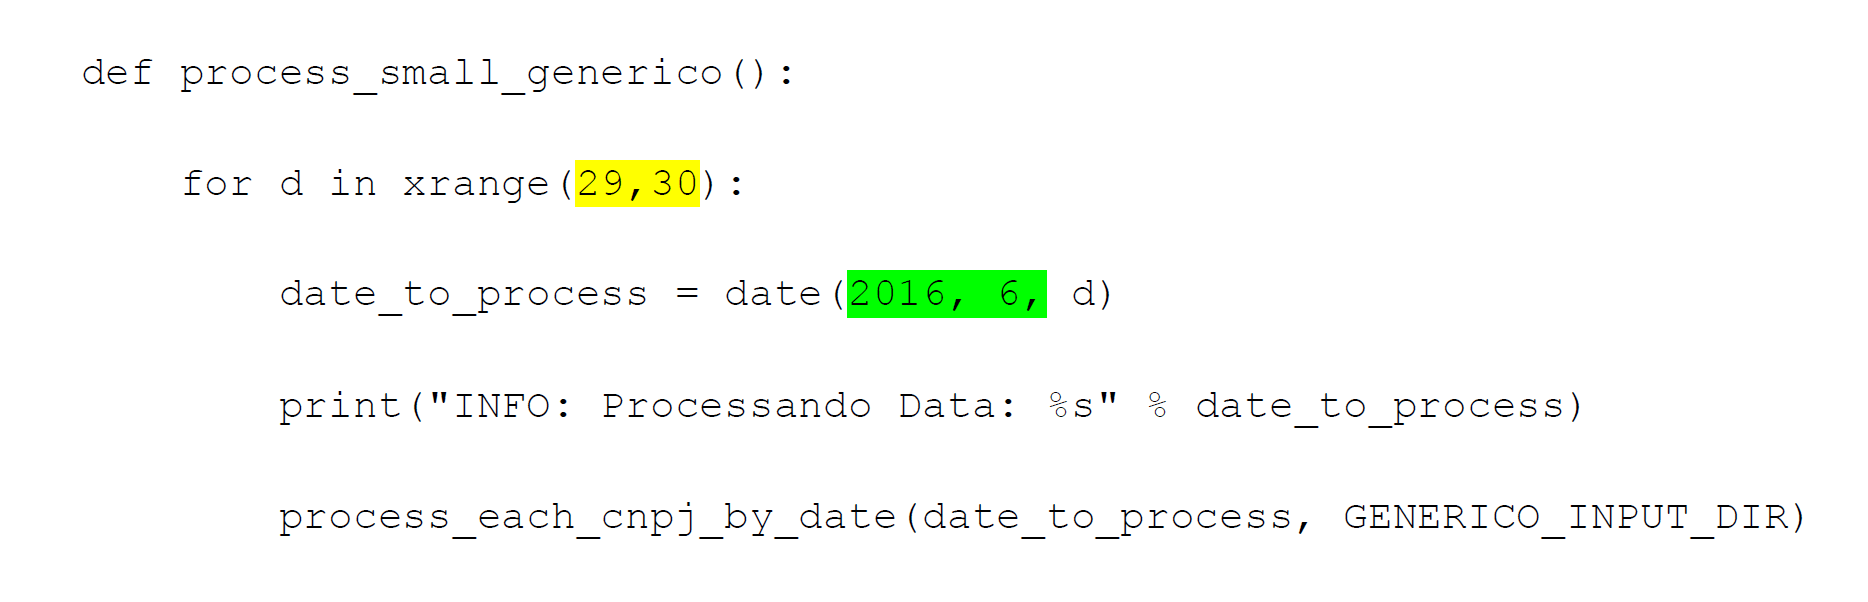
\includegraphics[width=1.0\textwidth]{genericos.png}
  \label{fig:genericos}
  \caption{Trecho de código a ser alterado}
\end{figure}

No exemplo da figura~\ref{fig:genericos} uma vez chamdo o $processa\_genericos.py$ pela linha de comando, processará \textbf{somente} o dia 29 do mês 6 de 2016.

Arquivos de logs com extensão \textbf{.log} serão gerados no mesmo diretório para auxiliar em caso de problemas.

O programa digere os dados da pasta \textbf{Cupons/processar (.NS)} e o resultado da digesão dos dados estarão na pasta \textbf{Cupons/processados (.csv, .pag).}



\section{Sugestão de testes}

\begin{itemize}
    \item Reprocesamento dos cupons Daruma.
    \item Troca de ECFs com venda de item.
    \item Troca de ECFs sem venda de item.
    \item Reprocessamento dos cupons Epson.
    \item Reprocessamento de cupons Sweda.
\end{itemize}

\end{document}               % End of document.